%%%%%%%%%%%%%%%%%%%%%%%%%%%%%%%%%%%%%%%%%

%---------------------------------------------------------------------------------------- 
%       Paquetes y configuraciones
%----------------------------------------------------------------------------------------

\documentclass[11pt, a4paper]{article} % Font size
\usepackage[sfmath]{kpfonts}
\renewcommand*\familydefault{\sfdefault}

\usepackage{charter} % Use the Charter font for the document text
\usepackage[utf8]{inputenc}
\usepackage[T1]{fontenc}
\usepackage[spanish,es-nolayout,es-nodecimaldot,es-tabla]{babel}
\usepackage{amsmath}
\usepackage{amsfonts}
\usepackage{amssymb,amsthm}
\usepackage{enumerate}
\usepackage{enumitem}
\usepackage{parskip}
\usepackage{listings}
\usepackage{nicefrac}
\usepackage{framed, color}
\usepackage{graphicx}
\usepackage[left=2cm,right=2cm,top=2.5cm,bottom=2cm]{geometry}
\usepackage[colorlinks = true]{hyperref} 
\usepackage{wrapfig}
\usepackage[font={footnotesize,it}]{caption}

%
%       Configuración de Problema y Proposición
%
\definecolor{db}{RGB}{0,128,128}                % Color de pregunta y respuesta
\definecolor{dg}{RGB}{128,0,128}                % Color de proposiciones y teoremas
\definecolor{dh}{RGB}{128,128,0}                % Color de preguntas adicionales
\definecolor{da}{RGB}{0,102,153}                % Color de direcciones electrónicas
\newtheorem{teo}{Teorema}

\newtheoremstyle{dotlessP}{1em}{\topsep}{\color{db}}{}{\color{db}\bfseries}{}{ }{}
\theoremstyle{dotlessP}
\newtheorem*{prob}{Problema:}

\newtheoremstyle{dotlessS}{1em}{\topsep}{\color{dg}}{}{\color{dg}\bfseries}{}{ }{}
\theoremstyle{dotlessS}
\newtheorem*{prop}{Proposición:}


% Comandos
\newcommand{\R}{\mathbb{R}}
\newcommand{\dsum}{\displaystyle \sum}
\newcommand{\yds}{\qquad\text{y}\qquad}
\DeclareMathOperator{\Dom}{Dom}
\DeclareMathOperator{\Ran}{Ran}
\DeclareMathOperator{\inv}{inv}


% Revisa para posible uso: http://principiae.be/pdfs/TUG-X-004-slideshow.pdf
%---------------------------------------------------------------------------------------------
%       Recursos desarrollados en la Comunidad virtual – Tutoría en línea
%---------------------------------------------------------------------------------------------

% Tipo de documento
\newcommand{\tipodedocumeto}{Curso de preparación al examen Ser bachiller}

% Autor
\newcommand{\autor}{Tania Bastidas}

% Editores
\newcommand{\editores}{Andrés Miniguano Trujillo y Juan Carlos Trujillo}

% Correos electrónicos
\newcommand{\email}{\href{mailto:taniabastidas5@hotmail.com}{\color{da}taniabastidas5@hotmail.com}}

\newcommand{\emaila}{\href{mailto:andres.miniguano@epn.edu.ec}{\color{da}andres.miniguano@epn.edu.ec}}

\newcommand{\emailb}{ y \href{mailto:jcto36@gmail.com}{\color{da}jcto36@gmail.com}}

% Fecha de creación de la pregunta
\newcommand{\creacion}{5 de abril de 2017}

% Fecha de publicación del recurso
\newcommand{\publicacion}{5 de abril de 2017}

% Título del recurso
\newcommand{\titulo}{Preguntas}


\usepackage{fancyhdr}
\pagestyle{fancy}
\renewcommand{\headrulewidth}{0pt}
\chead{\titulo}


\usepackage{lastpage}
\cfoot{\thepage\ de \pageref{LastPage}}


%----------------------------------------------------------------------------------------

\begin{document}\thispagestyle{empty}

\begin{center}

\includegraphics[width=0.5\linewidth]{logos.pdf}
\end{center}


\begin{flushleft}

\large
\rule{\textwidth}{1pt} \vspace{-1em} \par \noindent
\centerline{\LARGE                                      \tipodedocumeto                 } 
\vspace{-0.75cm} \par\noindent%
\rule{\textwidth}{1pt} \par \noindent
%
%
\setlength{\tabcolsep}{0pt}%
%
\begin{tabular}{l@{\hspace{1em}}l}%
        \textbf{Autor:}                 &        \autor \, (\email) \\
        \textbf{Editores:}               &        \editores                                \\
                                                & Proyecto CLAVEMAT              \\ 
                                                & Escuela Politécnica Nacional  \\
        \textbf{Email:}                  & \emaila                \emailb                                  \\
        \textbf{Creación:}               &  \creacion                             \\
        \textbf{Publicación:}            &  \publicacion
\end{tabular}%
\end{flushleft}
%
%
\rule{\textwidth}{1pt}  \vspace{-1em} \par \noindent
\centerline{\textbf{\Large              \titulo                 }} \vspace{-1em}
\rule{\textwidth}{1pt}  \vspace{1em} \par

%----------------------------------------------------------------------------------------
%       Contenidos
%----------------------------------------------------------------------------------------

\begin{enumerate}[label=\color{dg}\theenumi.]
        \setcounter{enumi}{20}
        \normalsize
        \item {\color{db}La sucesión permite generar códigos que faciliten la búsqueda de cada nuevo cliente en un almacén. ¿Cuál es el código que se asignó al cuarto cliente?
        
        \[
       	 3E,\, 6G,\, 12I, \,\dots\, , 48M
        \]
}
Nota que la sucesión contiene un número y una letra, donde el número siguiente es el doble del anterior y las letras van de dos en dos según el orden del alfabeto y desde la \(	E\) .

De este modo el siguiente código es: 
\[
	24k.
\]

   {\color{dh} La respuesta correcta es la 4.}
   
   
\item {\color{db}La serie representa el número diario de hojas que caen sobre una piscina, provenientes de . un árbol cercanos al iniciar a estación de otoño. ¿Cuántas hojas caerán sobre la piscina al octavo día?
        
        \[
      	  1,\, 5,\, 4, \,8,\,7,\,11, 10,\, \dots 
        \]
}   

A los términos de la sucesión se les puede agrupar alternando pares e impares
\[
	1,\,4, \,7,\,10 \qquad \text{y}\qquad 5,\, 8 , \, 11, \, \dots
\]

En ambas sucesiones, la distancia entre los términos es \(3\) y así el número siguiente es:
\[
	11 + 3 = 14.
\]


   {\color{dh} La respuesta correcta es la 3.}
   
 \item {\color{db}El concurso de una feria consiste en predecir el siguiente número que aparecerá en la ruleta. Si \(x\) es el próximo número en aparecer, ¿cuál es su valor?
 \begin{center}
  		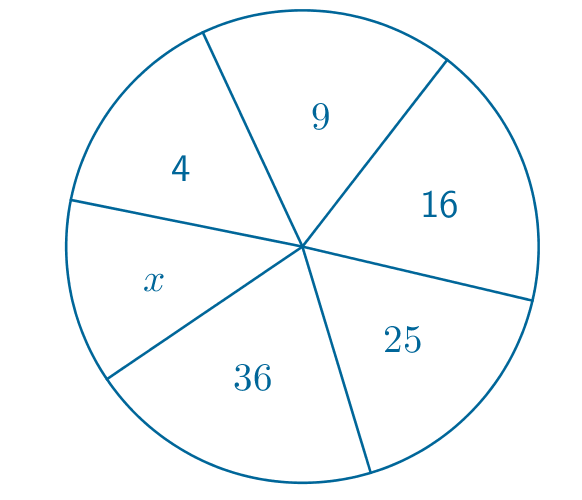
\includegraphics[scale=1]{SerBachiller23_fig1}
  \end{center}
}   
  Nota que los números de la rueda es una serie en donde, el número consecutivo se le obtiene sumando \(2\) más lo sumado anteriormente, es decir, que si sumo \(5\), al siguiente término se le suma \(7\), y al siguiente \(11\) y asi consecutivamente, entonces:
  \begin{align*}
  	x&= 36 + 13\\
    x&= 49.
  \end{align*}
  {\color{dh} La respuesta correcta es la 4.}
  
  \item {\color{db}La importación de un equipo cuesta \(\$ 600\), adicionalmente, se paga por transporte el \( 20 \%\). Sobre este nuevo valor se paga un \(5\%\) del valor del seguro. Identifique el valor total, en dólares,q ue se paga por el equipo importado.  
}   

Tienes que para la importación del equipo es \(\$ 600\), y que el \(20 \%\) de esta cantidad es para el pago del transporte; es decir
\[
	20\% (600)= 120,
\]
hasta ahora, la cantidad a pagar es:
\[
	600 + 120 = 720.
\]
Ahora, el valor a pagar del seguro corresponde
\[
	5\% (720)= 36.
\]
Por lotanto, el valor total a pagar es:
\[
	720 + 36 = 756.
\]
{\color{dh} La respuesta correcta es la 4.}

\item {\color{db}Paúl tiene \( \$25 \) para comprar comida para una reunión con sus amigos, así que desea comprar gaseosas (\( \$2 \) cada una) y chocolates (\( \$3 \) cada uno). Si Paúl decide comprar más gaseosas que chocolates, determine el gráfico que representa el conjunto de opciones que tiene Paúl para efectuar la compra. 
}
 \begin{center}
  		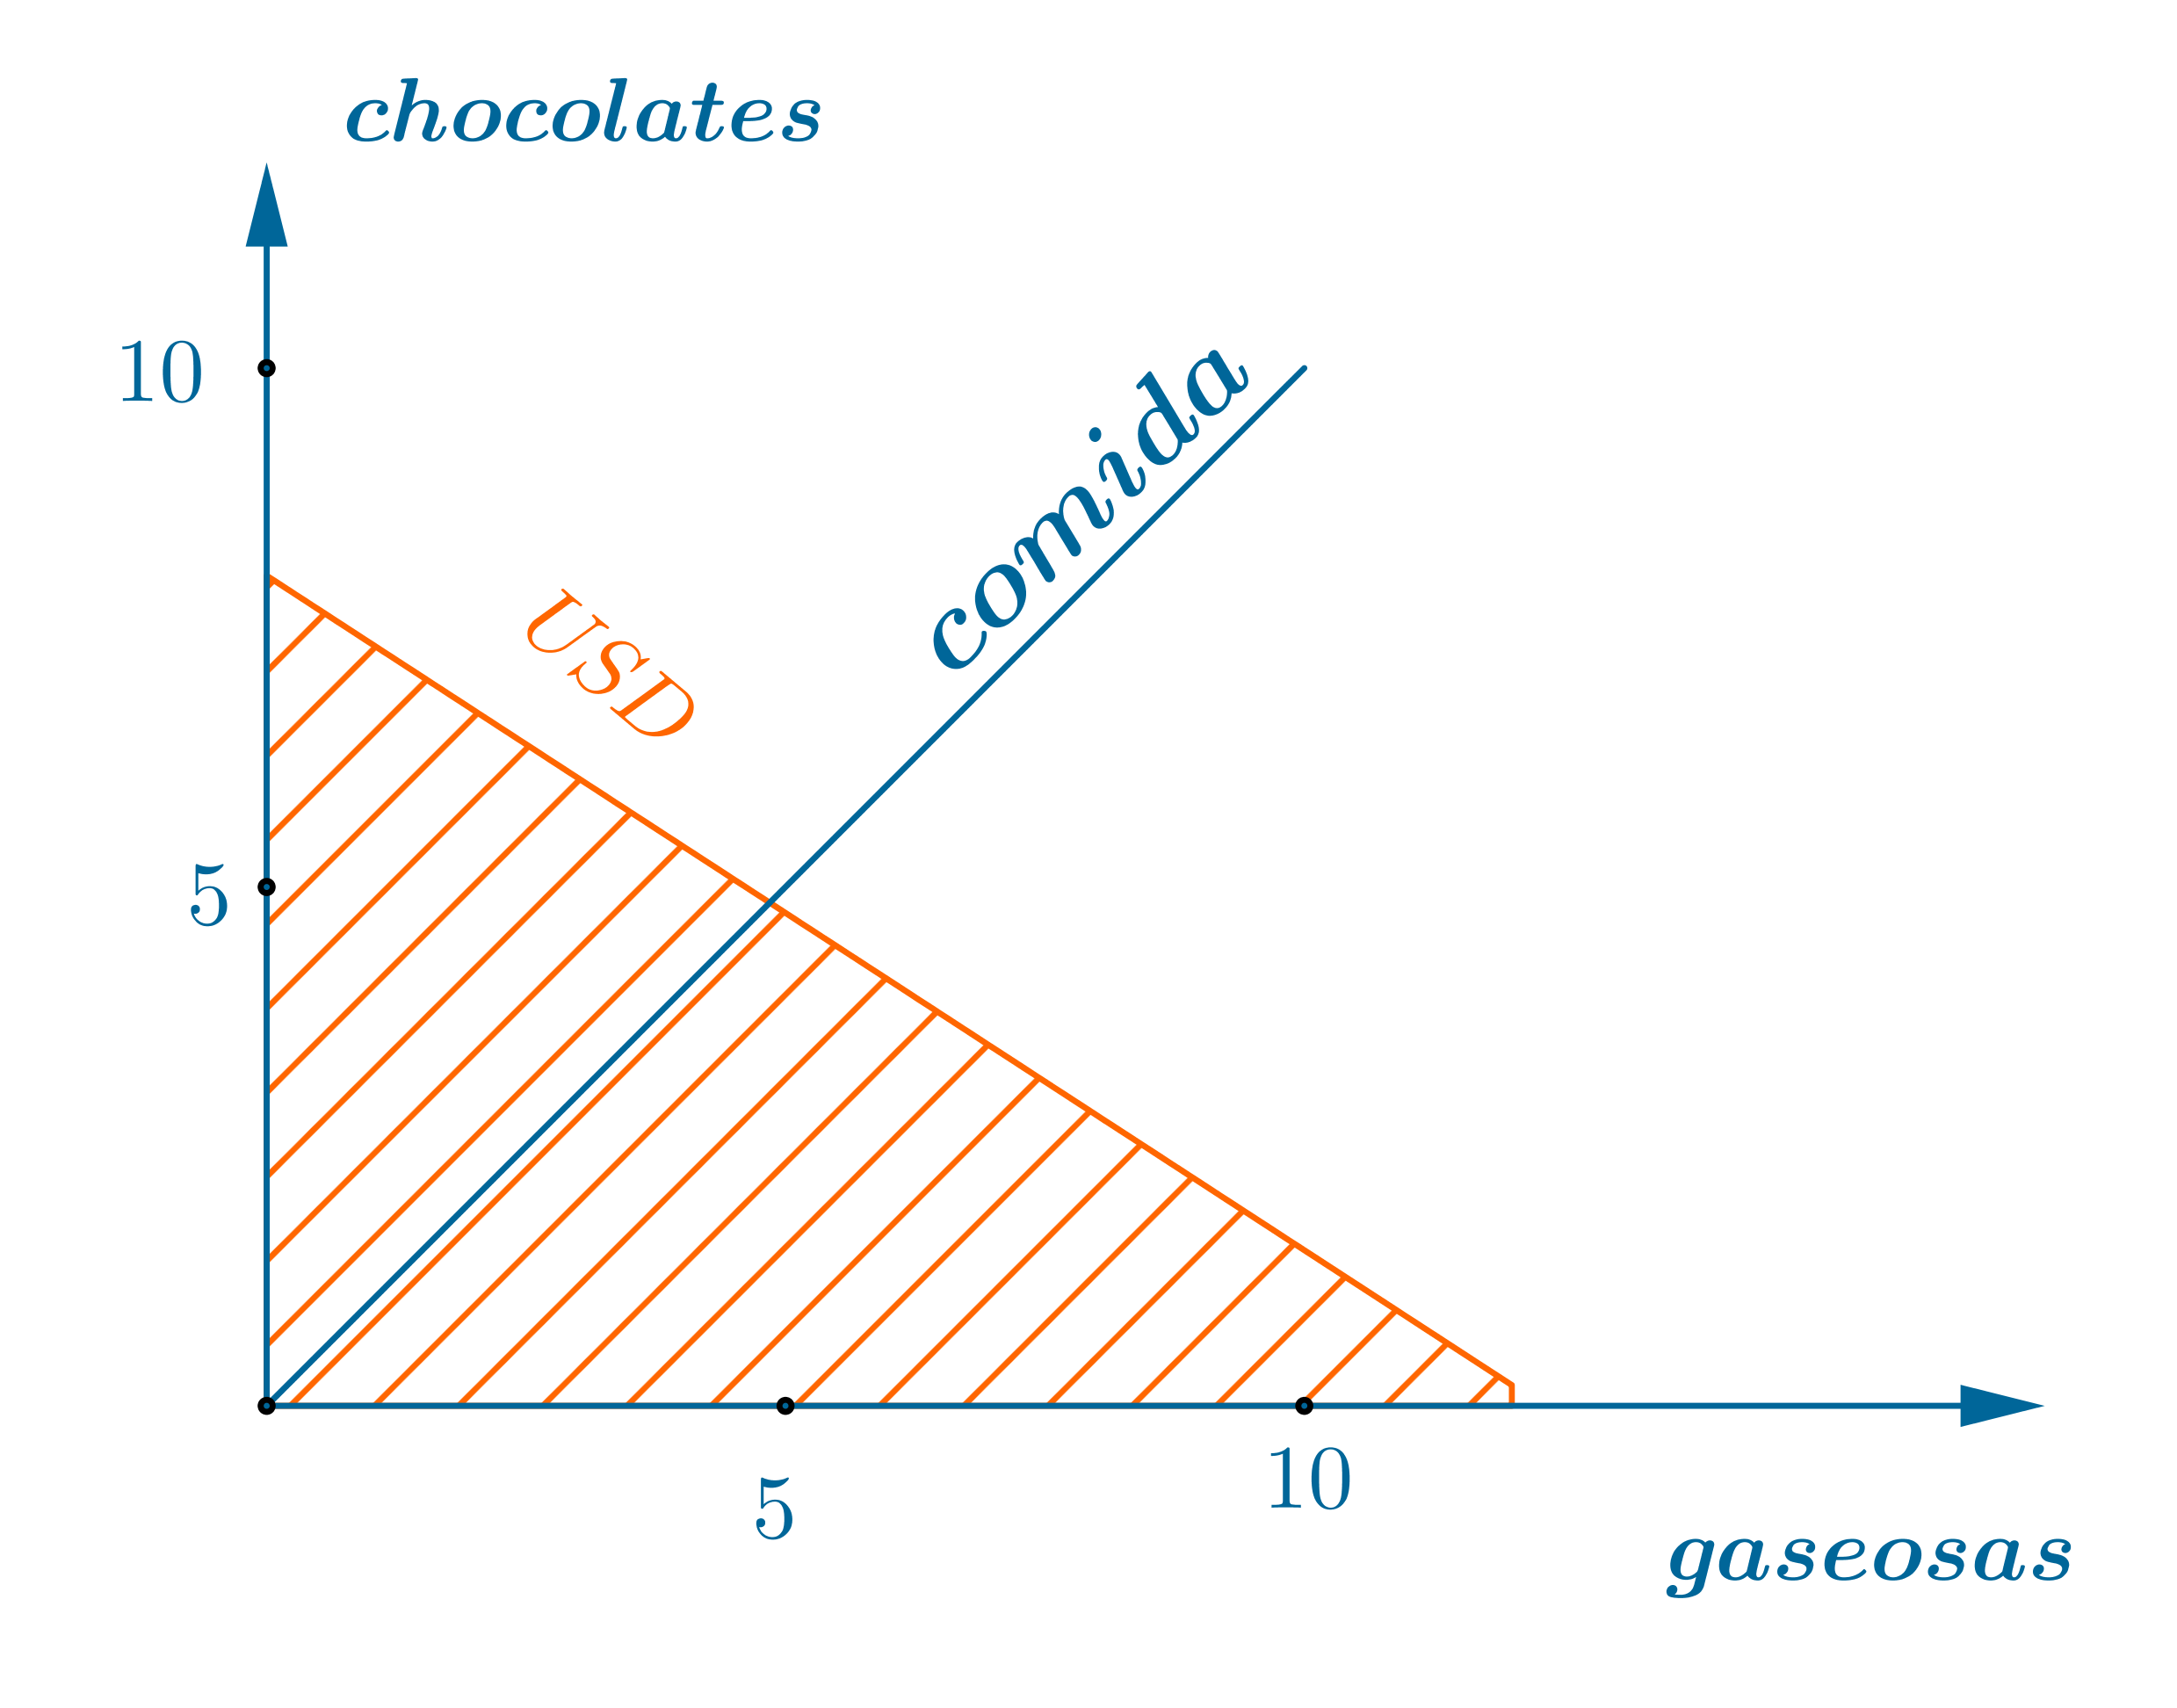
\includegraphics[scale=0.5]{SerBachiller25_fig1}
  \end{center}
  
  Nota que Paúl tiene \( \$25 \) 
  
  
  {\color{dh} La respuesta correcta es la 2.}
  \item[142] {\color{db}Identifique la figura que representa la incógnita
}
 \begin{center}
  		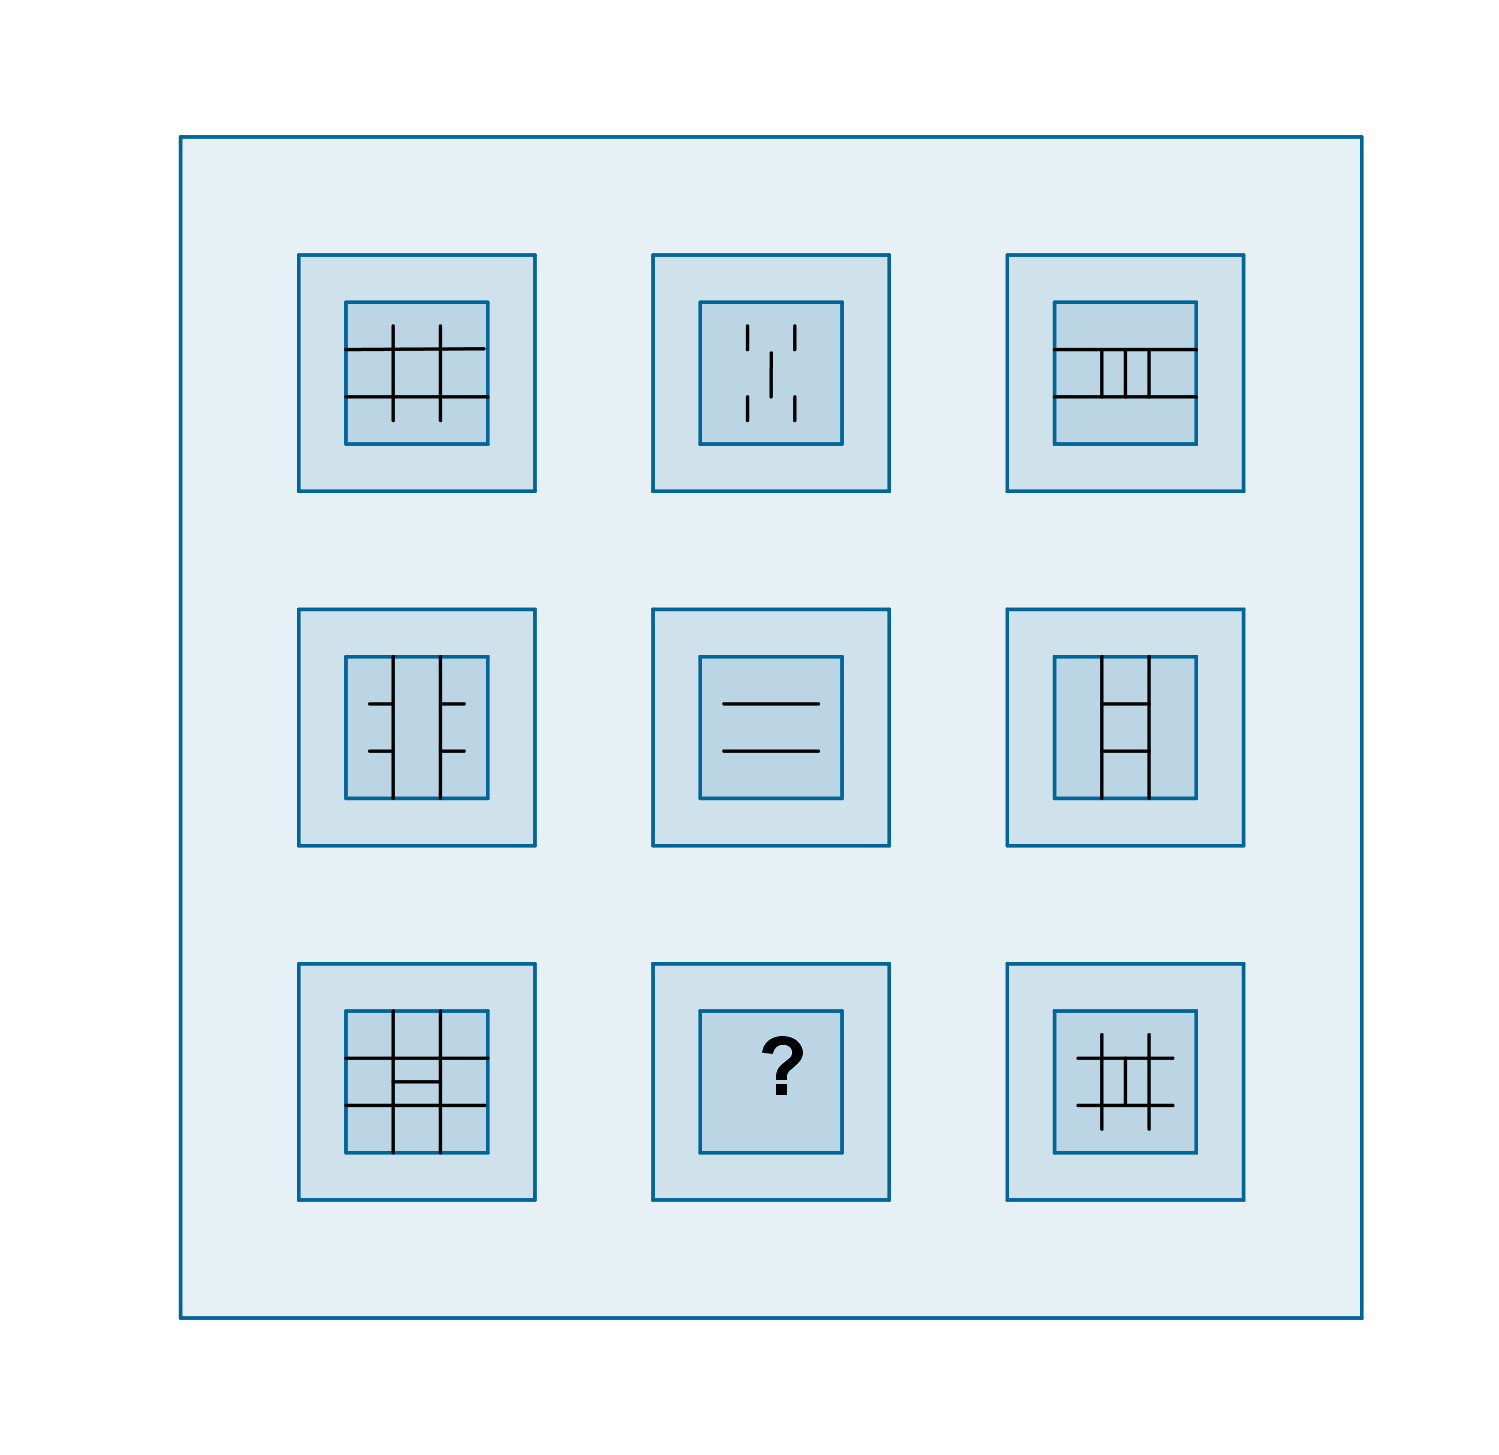
\includegraphics[scale=1]{SerBachiller142_fig1}
  \end{center}
 
  \begin{center}
  		
\includegraphics[scale=0.3]{SerBachiller142_fig2}
  \end{center}
  

  
  
  {\color{dh} La respuesta correcta es la 4.}
   \item[143] {\color{db}Identifique la figura que representa la incógnita
}
 \begin{center}
  		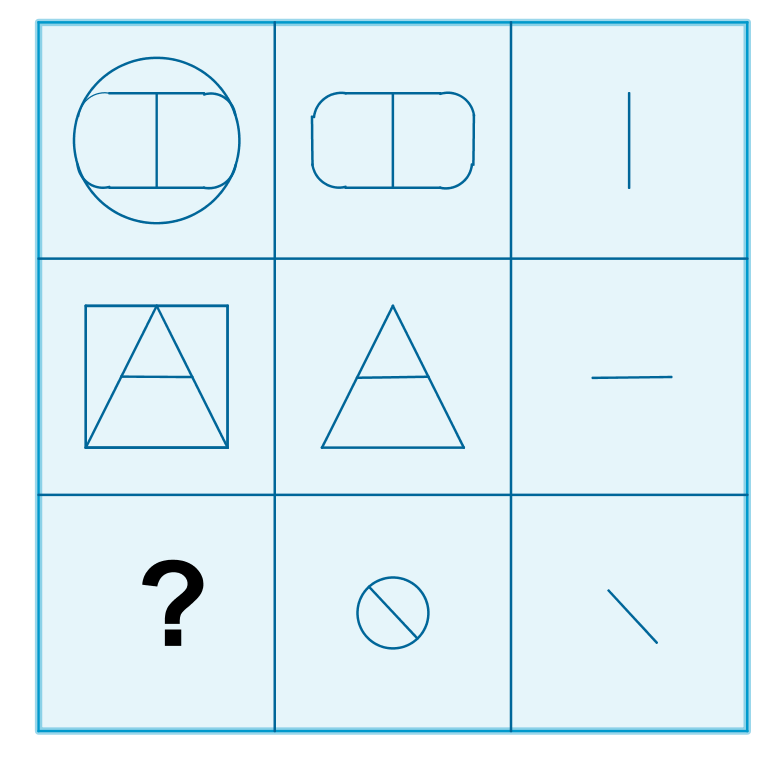
\includegraphics[scale=1]{SerBachiller143_fig1}
  \end{center}
 
  \begin{center}
  		
\includegraphics[scale=1]{SerBachiller143_fig2}
  \end{center}
  

  
  
  {\color{dh} La respuesta correcta es la 1.}
   
 %\begin{center}
       		 %\includegraphics[scale=1]%{SERBACHILLER_3png}
 % \end{center}
\end{enumerate}

\end{document}
